\documentclass[12pt, letterpaper]{article}
\usepackage[utf8]{inputenc}
\usepackage{amsmath}
\usepackage{graphicx}
\usepackage{geometry}
 \geometry{
 bottom=20mm,
 right=20mm,
 left=20mm,
 top=20mm,
 }

\newcommand{\pc}{\mbox{$\rm pc$}}
\newcommand{\kms}{\mbox{$\rm km\,s^{-1}$}}
\newcommand{\Msun}{\mbox{$\rm M_\odot$}}

\title{The Essentials of Molecular Clouds}
\author{Jiayi Sun}
\date{July 10, 2018}

\begin{document}

\maketitle

In the 1980s, the pioneering works done by Larson (1981) and Solomon et al. (1987)  offered a lot of insights on the structure and dynamical state of molecular clouds. The key results from these studies were the so-called ``Larson's relations''. Two of them are shown below:

\begin{figure}[htb]
\begin{center}
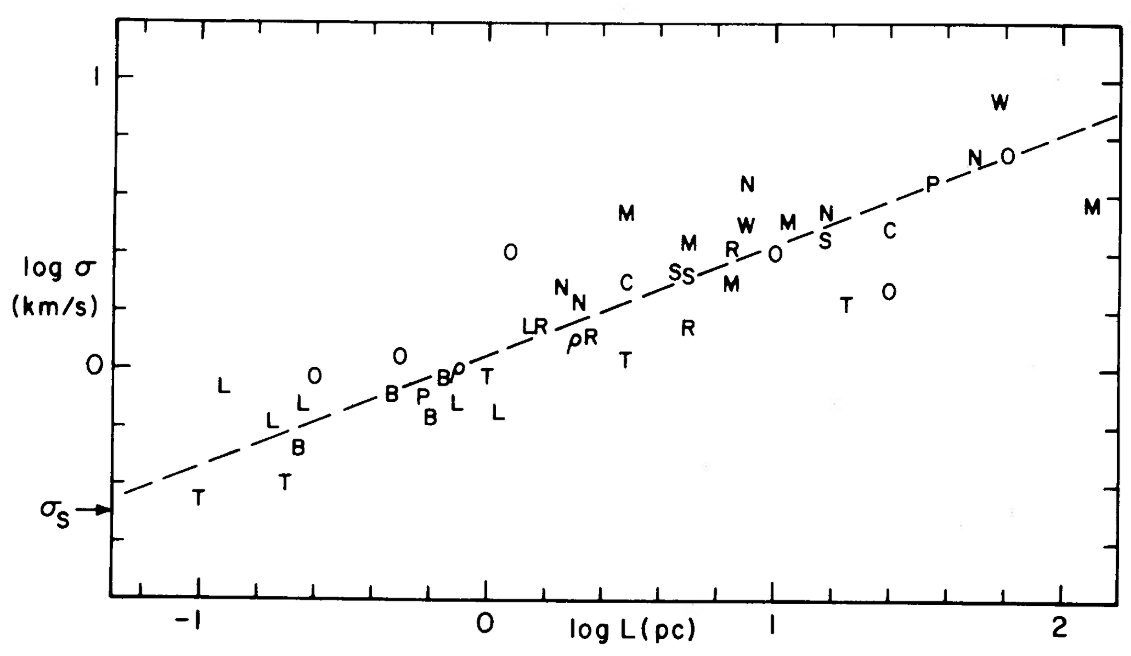
\includegraphics[width=0.60\textwidth]{1.png}
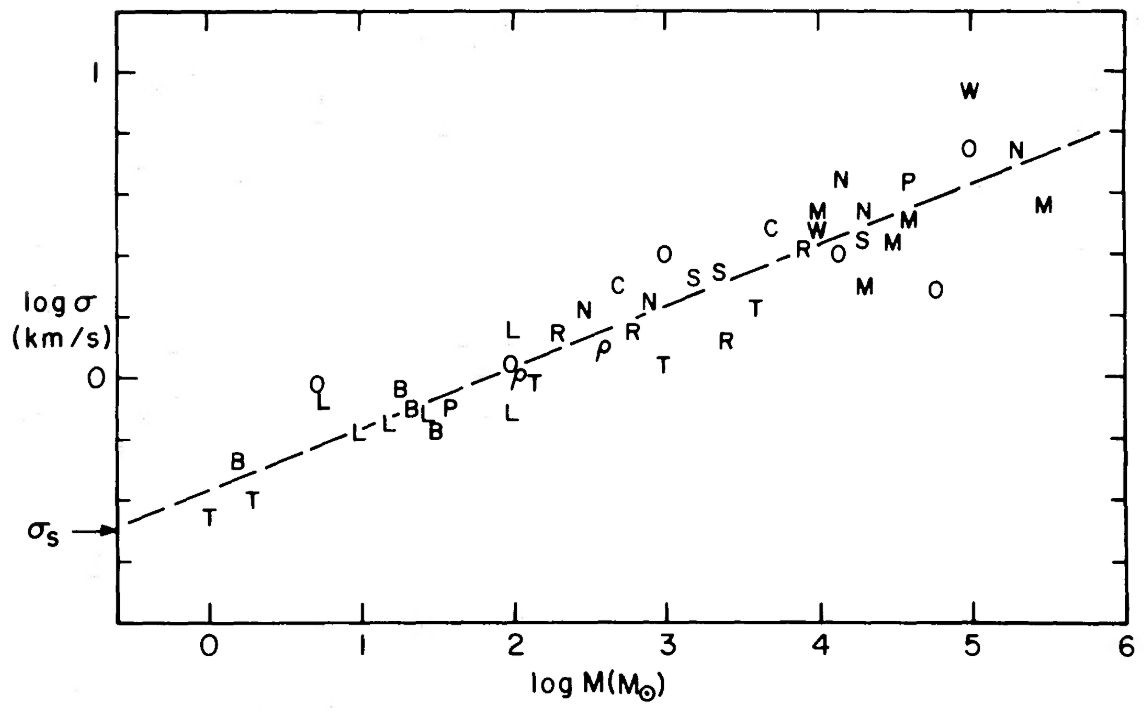
\includegraphics[width=0.61\textwidth]{2.png}
\caption{The size{--}line-width relation (top) and the mass{--}line-width relation (bottom), as reported by Larson (1981). {\bf We will adopt a slope $\approx 0.5$ for the former relation} (as suggested by Solomon et al. 1987), {\bf and slope $\approx 0.25$ for the latter} (though it looks more like 0.2 given these data). Note that $L$ stands for the ``maximum linear extent'' of each region identified as a cloud.}
\end{center}
\end{figure}

\begin{enumerate}

\item {\it What are the average surface densities of the clouds? Do they depend on cloud size?}

\item[$\Rightarrow$] One can rewrite Larson's relations as
\begin{align}
    \left( \frac{\sigma}{\;\kms} \right) \approx
    \left( \frac{L}{\pc} \right)^{0.5} \approx \left( \frac{M}{10^2\;\Msun} \right)^{0.25},
\end{align}
and thus the average surface density can be expressed as
\begin{align}
    \Sigma
    \approx \frac{M}{\pi (L/2)^2}
    \approx 10^2\;\Msun\,\pc^{-2},
\end{align}
which is not a function of cloud size.

This is one of the deductions from Larson's relations -- all molecular clouds have roughly the same surface density. However, later works have shown that this likely came from observational bias, as early observations were limited by sensitivity. Cloud surface density clearly varies across a galaxy and among galaxies (e.g., see Figure 13 in Leroy et al. 2015).

\item {\it What are the virial parameters of the clouds? Do they depend on cloud size? (Hint: for spherically symmetric objects with a given radial density profile, the virial parameter $\alpha_{\rm vir} \equiv 2K/U_g = 5\,\sigma^2 R/(f\,G M)$. Here $f$ is a dimensionless geometrical factor determined by the density profile, and it is typically of order unity.)}

\item[$\Rightarrow$] Substituting the $R$ and $M$ with Equation (1), we have
\begin{align}
    \alpha_{\rm vir}
    \approx \frac{5\,\sigma^2 L}{2\,G M}
    \approx \frac{5 \left(\frac{\sigma}{\kms}\right)^2 \left(\frac{\sigma}{\kms}\right)^2}{2 \times (4.3 \times 10^{-3}) \times 10^2 \left(\frac{\sigma}{\kms}\right)^4}
    \approx 5.8,
\end{align}
which, again, is not a function of cloud size.

This is yet another deduction from Larson's relations -- the ratio between molecular cloud kinetic energy and gravitational potential energy is roughly the same. Note that virialized objects have $\alpha_{\rm vir} \approx 1$, while marginally bound objects have $\alpha_{\rm vir} \approx 2$. More recent observations suggest that $\alpha_{\rm}$ is closer to 2, and the systematic uncertainty is still large.

\item {\it Consider CO molecules at 10 K: how does the thermal sound speed compare to the observed line width? And does this depend on the linear scale that we consider?}

\item[$\Rightarrow$] The thermal sound speed can be expressed as
\begin{align}
    \sigma_{\rm S}
    \approx \sqrt{\frac{k_{\rm B}T}{m_{\rm CO}}}
    \approx \sqrt{\frac{1.38 \times 10^{-23} \times 10}{28 \times 1.66 \times 10^{-27}}}\rm\;m\,s^{-1}
    \approx 50\rm\;m\,s^{-1}.
\end{align}
This is much smaller than the $\sim \kms$ CO line width that we observe on pc scale.

This comparison, together with the fact that CO line width scales with linear size, suggests that turbulence broadening is much more important than thermal broadening on pc scale. However, if the size{--}line-width relation still holds on smaller scale, thermal motion becomes dominant as one goes down to sub-pc scale.

\item {\it Turbulence is not long-lived. The kinetic energy associated with turbulence flows from large scales to small scales (also known as ``turbulence cascade''), and eventually it will dissipate and be converted to thermal energy. It is suggested that, if there is no source that generates turbulence, all the energy in turbulence will dissipate in one turbulence crossing time $\tau_{\rm cross} \sim L/\sigma$. Calculate the amount of dissipated energy per unit time per unit mass, and keep its scaling relation with cloud size $L$.}

\item[$\Rightarrow$] The total kinetic energy of a molecular cloud is $K \approx 3/2M\sigma^2$.
% \begin{align}
%     K \approx \frac{3}{2}M\sigma^2
%     \approx 1.5\;(\kms)^2 \left(\frac{L}{\pc}\right) M.
% \end{align}
Since most of the kinetic energy is associated with turbulence, the energy dissipation rate per unt mass is thus
\begin{align}
    \frac{K}{M\tau_{\rm cross}}
    \approx \frac{3\,\sigma^3}{2L}
    \approx 1.5\;(\kms)^3\;\pc^{-1} \left(\frac{L}{\pc}\right)^{0.5}
    \approx 5 \times 10^{-4}\rm\;ergs\,g^{-1}\,s^{-1} \left(\frac{L}{\pc}\right)^{0.5}.
\end{align}

\item {\it It seems that turbulence cascade is an efficient heating source. Will CO line cooling be efficient enough to balance it? (The CO cooling rate, according to Barbara's ISM textbook, is on average $\sim 10^{-27}\rm\;ergs\;s^{-1}$ per hydrogen nucleus at 10 K.)}
 
\item[$\Rightarrow$] The CO cooling rate per unit mass is
\begin{align}
    10^{-27}\rm\;ergs\;s^{-1} / (1.7 \times 10^{-24}\rm\;g) \approx 6 \times 10^{-4}\rm\;ergs\,g^{-1}\,s^{-1}.
\end{align}
The agreement is actually better than what we would expect. Generally speaking, CO is the dominant coolant in the density range $n \approx 10^3-10^5\rm\;cm^{-3}$, whereas shock heating is the dominant heating source for $n \geq 10^4\rm\;cm^{-3}$ (see Glover \& Clark 2012). Therefore, for most regions inside a molecular cloud (excluding the dense clumps), we do expect a good match between shock heating rate and CO line cooling rate.

\end{enumerate}

\section*{References}

\begin{itemize}
    \item Glover S. C. O., Clark P. C., 2012, MNRAS, 412(1), 9
    \item Larson R., 1981, MNRAS, 194(4), 809
    \item Leroy A. K., Bolatto A. D., Ostriker E. C., et al., 2015, ApJ, 81, 25
    \item Solomon P. M., Rivolo A. R., Barrett J., \& Yahil A., 1987, ApJ, 319, 730
\end{itemize}

\end{document}
